\begin{figure}[t]
\centering
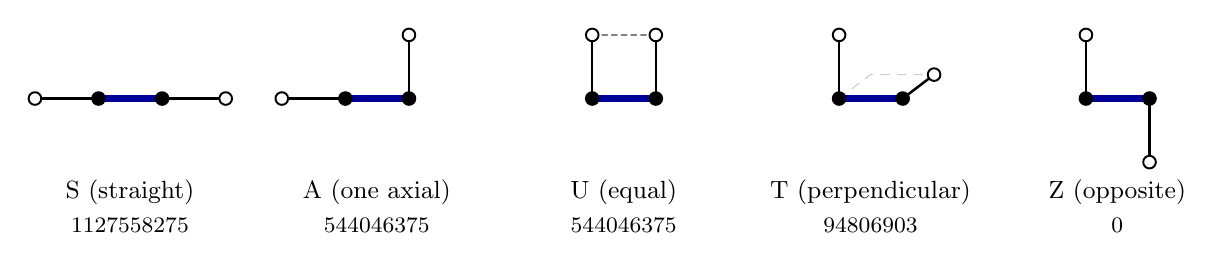
\begin{tikzpicture}[scale=0.95,line cap=round,line join=round]
\draw[black,line width=0.9pt] (-0.850,0.000) -- (0.000,0.000);
\draw[black,line width=0.9pt] (0.850,0.000) -- (1.700,0.000);
\draw[blue!60!black,line width=2.2pt] (0.000,0.000) -- (0.850,0.000);
\filldraw[fill=white,draw=black,line width=0.7pt] (-0.850,0.000) circle (2.4pt);
\filldraw[fill=black,draw=black,line width=0.7pt] (0.000,0.000) circle (2.4pt);
\filldraw[fill=black,draw=black,line width=0.7pt] (0.850,0.000) circle (2.4pt);
\filldraw[fill=white,draw=black,line width=0.7pt] (1.700,0.000) circle (2.4pt);
\node[font=\small] at (0.420,-1.25) {$\mathrm{S}$ (straight)};
\node[font=\footnotesize] at (0.420,-1.7) {$1127558275$};
\draw[black,line width=0.9pt] (2.450,0.000) -- (3.300,0.000);
\draw[black,line width=0.9pt] (4.150,0.000) -- (4.150,0.850);
\draw[blue!60!black,line width=2.2pt] (3.300,0.000) -- (4.150,0.000);
\filldraw[fill=white,draw=black,line width=0.7pt] (2.450,0.000) circle (2.4pt);
\filldraw[fill=black,draw=black,line width=0.7pt] (3.300,0.000) circle (2.4pt);
\filldraw[fill=black,draw=black,line width=0.7pt] (4.150,0.000) circle (2.4pt);
\filldraw[fill=white,draw=black,line width=0.7pt] (4.150,0.850) circle (2.4pt);
\node[font=\small] at (3.720,-1.25) {$\mathrm{A}$ (one axial)};
\node[font=\footnotesize] at (3.720,-1.7) {$544046375$};
\draw[black!50,dash pattern=on 2pt off 1.5pt] (6.600,0.850) -- (7.450,0.850);
\draw[black,line width=0.9pt] (6.600,0.850) -- (6.600,0.000);
\draw[black,line width=0.9pt] (7.450,0.000) -- (7.450,0.850);
\draw[blue!60!black,line width=2.2pt] (6.600,0.000) -- (7.450,0.000);
\filldraw[fill=white,draw=black,line width=0.7pt] (6.600,0.850) circle (2.4pt);
\filldraw[fill=black,draw=black,line width=0.7pt] (6.600,0.000) circle (2.4pt);
\filldraw[fill=black,draw=black,line width=0.7pt] (7.450,0.000) circle (2.4pt);
\filldraw[fill=white,draw=black,line width=0.7pt] (7.450,0.850) circle (2.4pt);
\node[font=\small] at (7.020,-1.25) {$\mathrm{U}$ (equal)};
\node[font=\footnotesize] at (7.020,-1.7) {$544046375$};
\draw[black!20,dashed] (9.900,0.000) -- (10.320,0.320) -- (11.170,0.320);
\draw[black,line width=0.9pt] (9.900,0.850) -- (9.900,0.000);
\draw[black,line width=0.9pt] (10.750,0.000) -- (11.170,0.320);
\draw[blue!60!black,line width=2.2pt] (9.900,0.000) -- (10.750,0.000);
\filldraw[fill=white,draw=black,line width=0.7pt] (9.900,0.850) circle (2.4pt);
\filldraw[fill=black,draw=black,line width=0.7pt] (9.900,0.000) circle (2.4pt);
\filldraw[fill=black,draw=black,line width=0.7pt] (10.750,0.000) circle (2.4pt);
\filldraw[fill=white,draw=black,line width=0.7pt] (11.170,0.320) circle (2.4pt);
\node[font=\small] at (10.320,-1.25) {$\mathrm{T}$ (perpendicular)};
\node[font=\footnotesize] at (10.320,-1.7) {$94806903$};
\draw[black,line width=0.9pt] (13.200,0.850) -- (13.200,0.000);
\draw[black,line width=0.9pt] (14.050,0.000) -- (14.050,-0.850);
\draw[blue!60!black,line width=2.2pt] (13.200,0.000) -- (14.050,0.000);
\filldraw[fill=white,draw=black,line width=0.7pt] (13.200,0.850) circle (2.4pt);
\filldraw[fill=black,draw=black,line width=0.7pt] (13.200,0.000) circle (2.4pt);
\filldraw[fill=black,draw=black,line width=0.7pt] (14.050,0.000) circle (2.4pt);
\filldraw[fill=white,draw=black,line width=0.7pt] (14.050,-0.850) circle (2.4pt);
\node[font=\small] at (13.620,-1.25) {$\mathrm{Z}$ (opposite)};
\node[font=\footnotesize] at (13.620,-1.7) {$0$};
\end{tikzpicture}
\caption{The five shapes of a triple of consecutive path bonds (\cref{def:shape}). The middle bond, whose endpoints are the two hubs, is drawn thick. The numbers are the shape charges $10^{12}w_\tau$ of \cref{tab:shapes}. In shape $\mathrm U$ the two outer vertices span a chord (dashed).}
\label{fig:shapes}
\end{figure}
